\documentclass[aspectratio=169]{beamer}
\setbeamertemplate{navigation symbols}{}
\usepackage{color,amsmath,comment, subfigure}
\usepackage{booktabs}
\usepackage{url}

%\setbeameroption{show notes}

%%%%%%%%%%%%%%%%%%%%%%%%%%
\title[]{Lecture 5: Degree distributions and power laws}
\author[]{Matthew J. Salganik}
\institute[]{Sociology 204: Social Networks, Spring 2021\\Princeton University}
\date[]{
2/2: Scale-free networks: implications, empirical work, and additional modeling

\vfill

\begin{flushleft}
\vspace{0.7in}

\includegraphics[width=0.05\textwidth]{figures/cc.png}
\end{flushleft}
}

\begin{document}
%%%%%%%%%%%%%%%%%%%%%%%%%%%
\frame{\titlepage}
%%%%%%%%%%%%%%%%%%%%%%%%%%%
\begin{comment}
\begin{frame}

SWBAT:
\begin{enumerate}
\item recognize networks that are scale-free and networks that are not scale-free
\item explain the data generating process for scale-free networks
\item explain the abstract similarity between Watts and Strogatz and Barabasi and Albert 
\end{enumerate}

\end{frame}
\end{comment}
%%%%%%%%%%%%%%%%%%%%%%%%
\begin{frame}

Follow up work:
\begin{itemize}
\item Implications
\item Empirical
\item Modeling
\end{itemize}

\note{
Most of this you have not read, but it should help you understand why what you read is interesting and important
}

\end{frame}
%%%%%%%%%%%%%%%%%%%%%%%%%%%
\begin{frame}
\frametitle{Implication}

\begin{center}
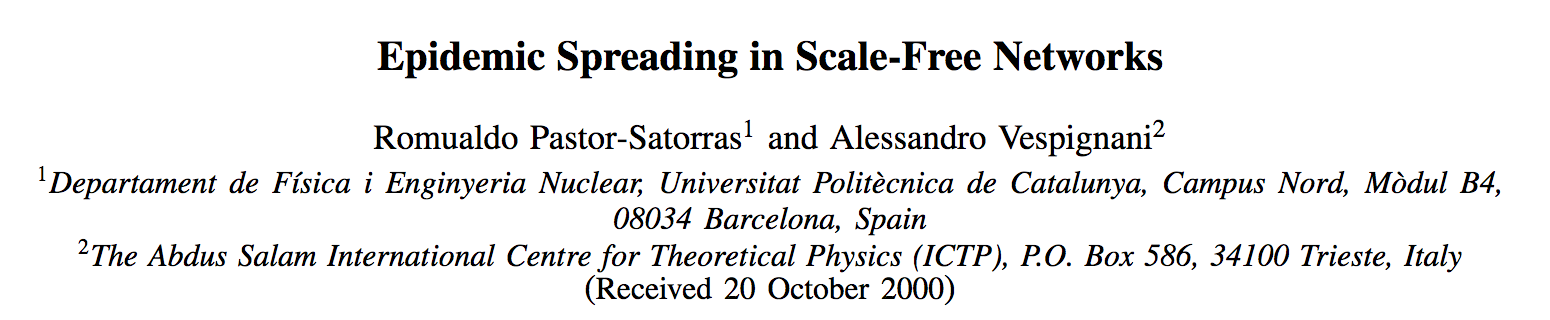
\includegraphics[width=\textwidth]{figures/pastor_satorras_epidemic_2001_title}
\end{center}

\pause

\begin{itemize}
\item Diseases are harder to stop when spreading in scale-free networks
\end{itemize}

\vfill
\url{http://dx.doi.org/10.1103/PhysRevLett.86.3200}

\note{
Diseases spread very differently on power law networks than ER random graph
In scale free network: absence of epidemic threshold. Roughly imagine that there is one person at person that interacts with everyone.  If someone gets sick, then the hub will get sick, then everyone many people will get sick
}

\end{frame}
%%%%%%%%%%%%%%%%%%%%%%%%%%%
\begin{frame}
\frametitle{Implication}

\begin{center}
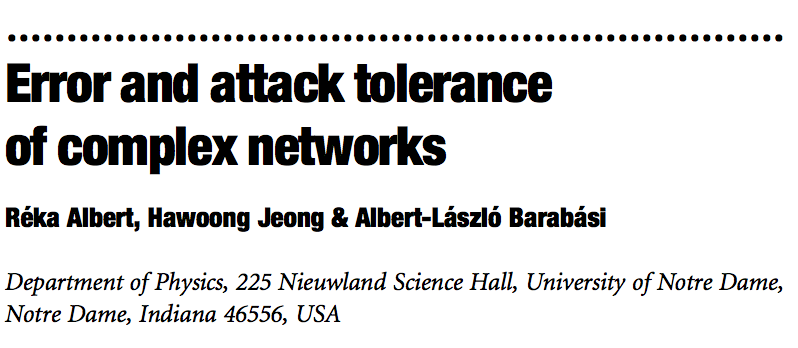
\includegraphics[width = 0.95\textwidth]{figures/albert_error_2000_title}
\end{center}

\vfill
\url{http://dx.doi.org/10.1038/35019019}

\end{frame}
%%%%%%%%%%%%%%%%%%%%%%%%%%%
%\begin{frame}
%\frametitle{Implication}
%
%\begin{center}
%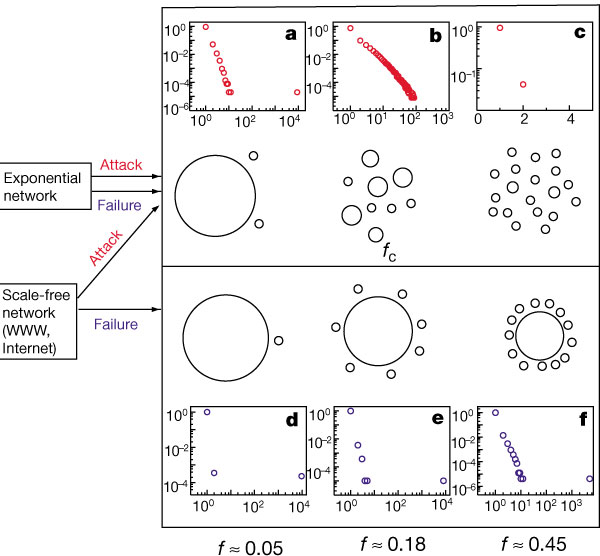
\includegraphics[height = 0.80\textheight]{figures/albert_error_2000_fig4}
%\end{center}
%
%
%\end{frame}
%%%%%%%%%%%%%%%%%%%%%%%%%%%
\begin{frame}
\frametitle{Implication}

\begin{center}
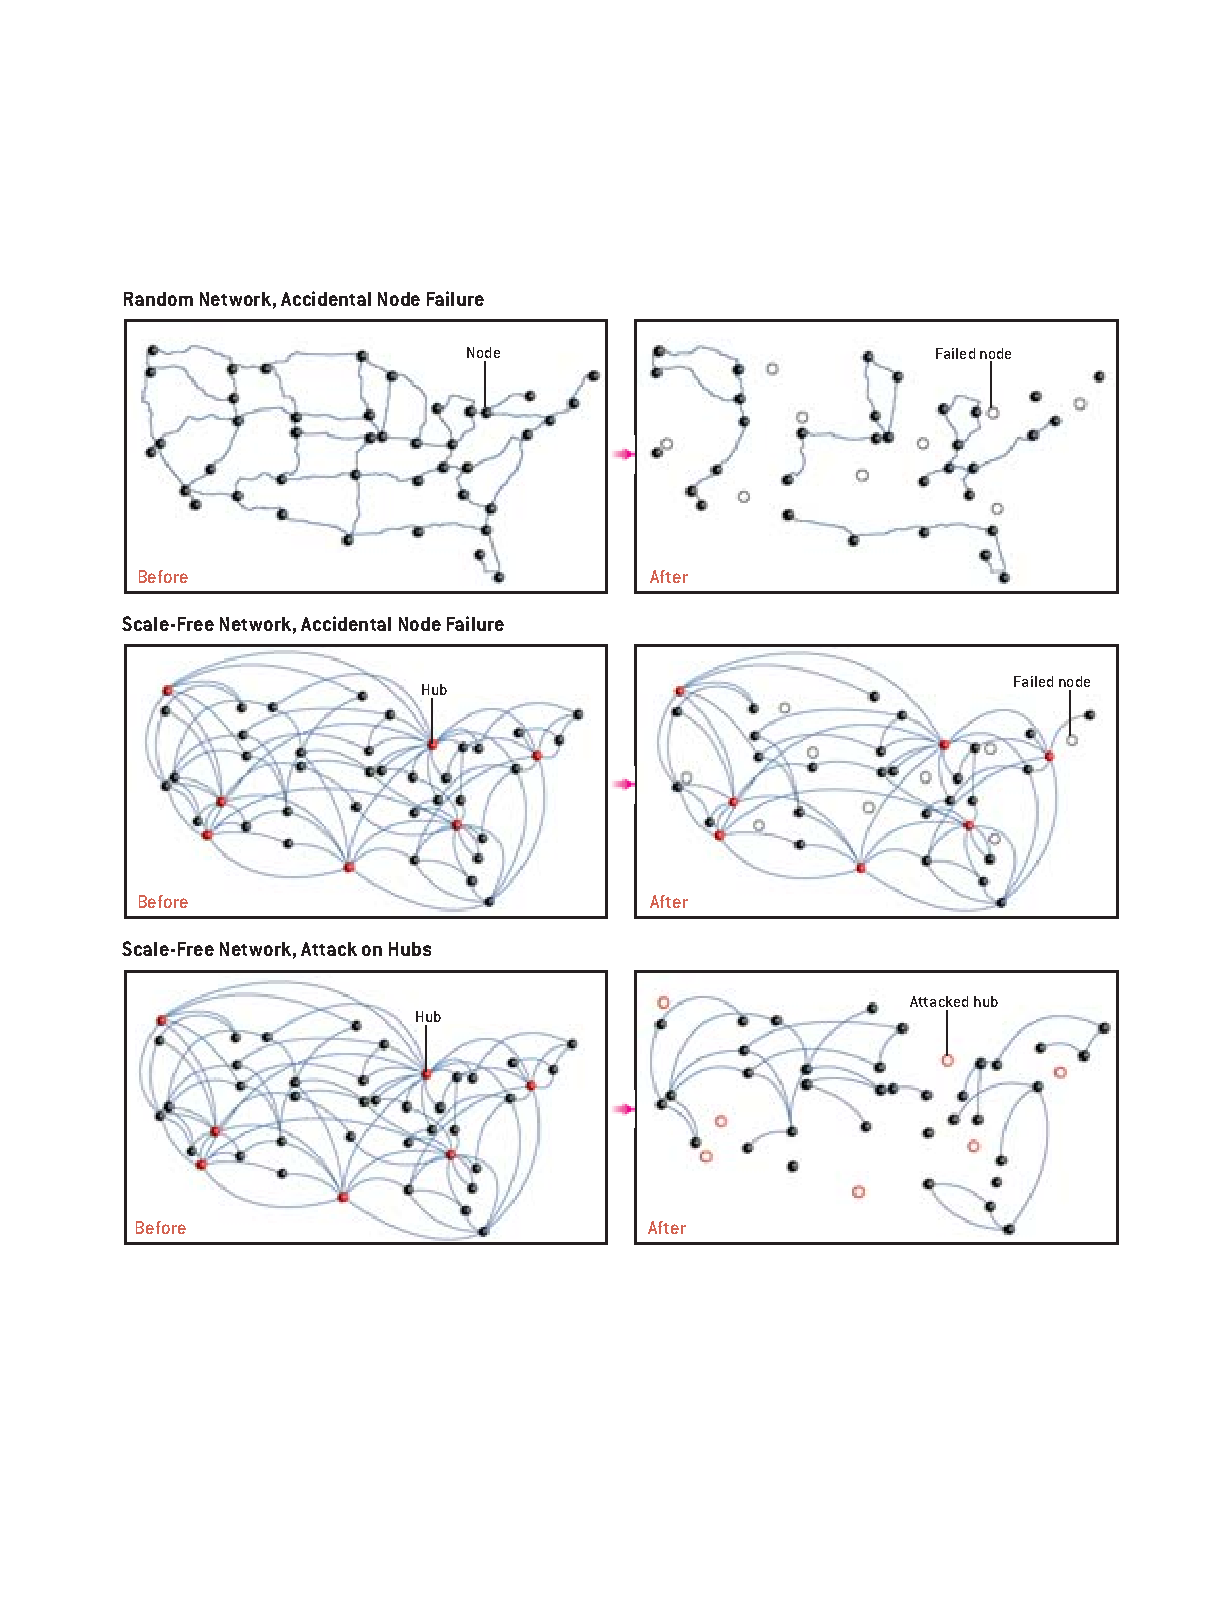
\includegraphics[height = 0.80\textheight]{figures/barabasi_scale-free_2003_robust}
\end{center}

\end{frame}
%%%%%%%%%%%%%%%%%%%%%%%%%%%
\begin{frame}
\frametitle{Emprical}

\begin{center}
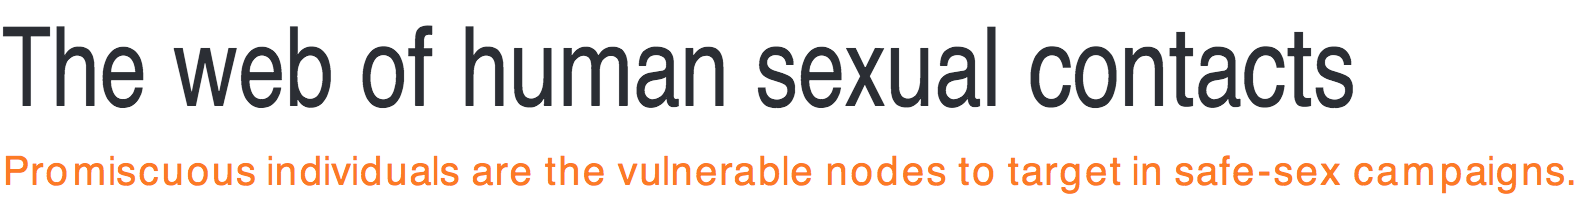
\includegraphics[width = 0.95\textwidth]{figures/liljeros_web_2001_title}
\end{center}

\vfill
\url{https://doi.org/10.1038/35082140}

\end{frame}
%%%%%%%%%%%%%%%%%%%%%%%%%%%
\begin{frame}
\frametitle{Emprical}

\begin{center}
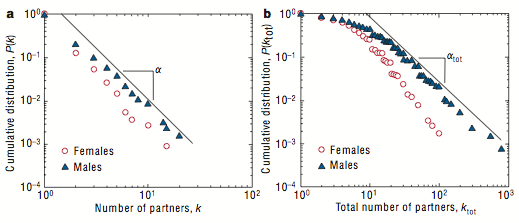
\includegraphics[width = 0.95\textwidth]{figures/liljeros_web_2001_fig2}
\end{center}

\note{
% Before talking about diseases let talk about information.

%Tulips arrived in Belgium from Turkey along with a shipment of cloth.  The merchant who received them planted them and discovered that they produced an unusually beautiful flower at which point he asked his friend Joris Rye what to make of them.  Rye didn't know by asked his fellow botinist Carolus Clusius.  Clusius was a hub.  It is estimated that he wrote some 4,000 letters in his life to botanists all over Europe.  He spoke 9 languages and was instruments in spreading the flower over the Continent (source: Tulipomania by Mike Dash). ALSO MENTION SCHEDULING CONSTRAINTS.  The role of hubs in social spreading is highly contested as we will read later in the semester.

If there is time, talk about the difference between men and women. Men over-report, women under-report, sex workers not included in surveys.

% Also, talk about how degree distribution is just a small part of network structure.

Given that the sexual network are power law, given that diseases spread differently on power law networks, and given that power law are susceptible to targeted attack, maybe we should target hubs.

Also, why this was so nasty.

Obviously we are not going to get into the details of who messed up their statistics, but I think the point that degree distribution is not everything is clearly right.  I also think the response from Jones and Handcock was pretty aggressive because Liljeros et al. made some pretty important claims about public health based on very limited data.  ``To justify using radically different prevention strategies for sexually transmitted infections, strong evidence is needed that current strategies will be ineffective.  Results based on unverified mathematical assumptions will about network structure do no come close to meeting that standard.  Such data provide no new insights for epidemiology and conclusions drawn from them could jeopardize campaigns to eliminate sexually transmitted infections worldwide.'' \\

Should we refocus our prevention strategy?  Not necessarily?  We'll read more about sexual networks later, but they have additional structure beyond just degree distribution (for example bridge populations).
}

\end{frame}
%%%%%%%%%%%%%%%%%%%%%%%%%%%
%\begin{frame}
%\frametitle{Empirical}
%
%\begin{center}
%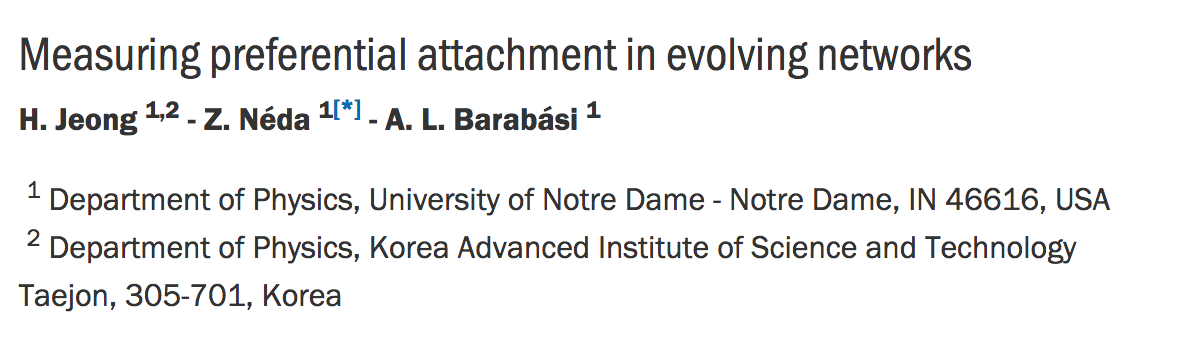
\includegraphics[width=\textwidth]{figures/jeong_measuring_2003_title}
%\end{center}
%
%\vf
%\url{http://iopscience.iop.org/0295-5075/61/4/567}
%
%\note{
%Measures growth process directly
%}
%
%\end{frame}
%%%%%%%%%%%%%%%%%%%%%%%%%%%
\begin{frame}
\frametitle{Empirical}

\begin{center}
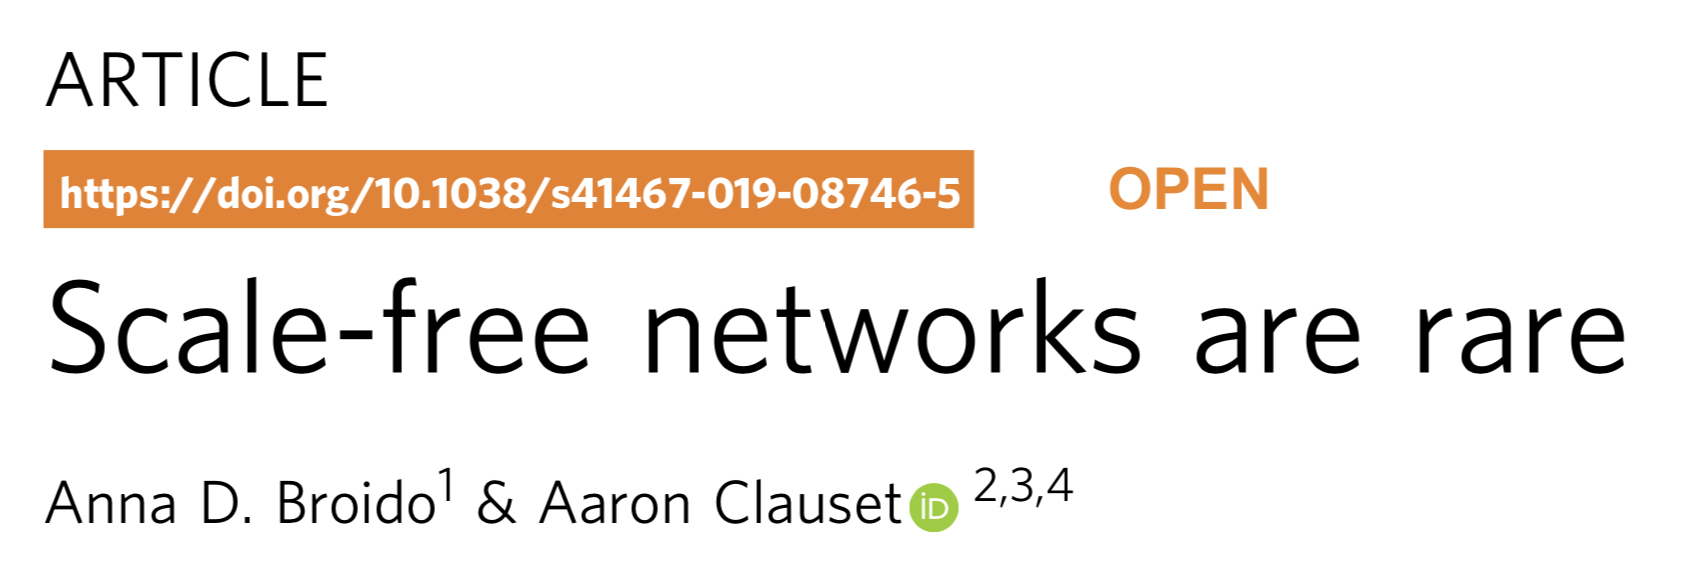
\includegraphics[width=0.6\textwidth]{figures/broido_scale-free_2019_title}
\end{center}

\begin{itemize}
\item Formal definitions of scale-free networks: Super-weak, weakest, weak, strong, strongest \pause
\item Analyzed nearly 1,000 social, biological, technological, transportation, and information networks \pause
\item Strongest form of scale-free structure is very rare \pause
\item Social networks seem least scale-free, whereas technical and biological seem more scale-free \pause
\end{itemize}
\vfill
\url{https://doi.org/10.1038/s41467-019-08746-5}

\end{frame}
%%%%%%%%%%%%%%%%%%%%%%%%%%%
\begin{frame}
\frametitle{Empirical}

\begin{center}
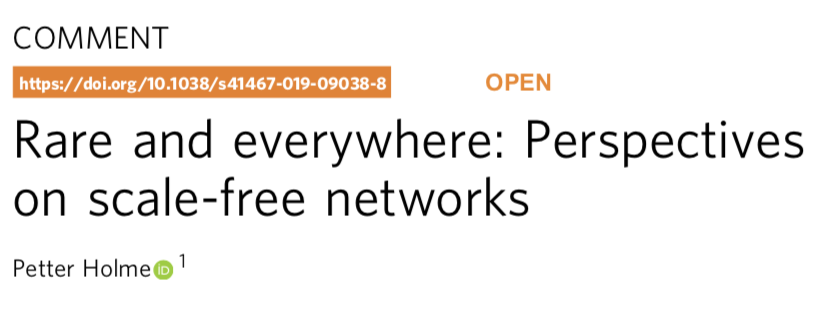
\includegraphics[width=\textwidth]{figures/holme_rare_2019_title}
\end{center}

\vfill
\url{https://doi.org/10.1038/s41467-019-09038-8}

\note{
Networks with skewed degree distributions are common
Skewed degree distribution is important for a variety of reasons
Empirically observed networks with power law degree distribution are rare, especially for social networks
}


\end{frame}
%%%%%%%%%%%%%%%%%%%%%%%%%%%
\begin{frame}
\frametitle{Modeling}

\begin{center}
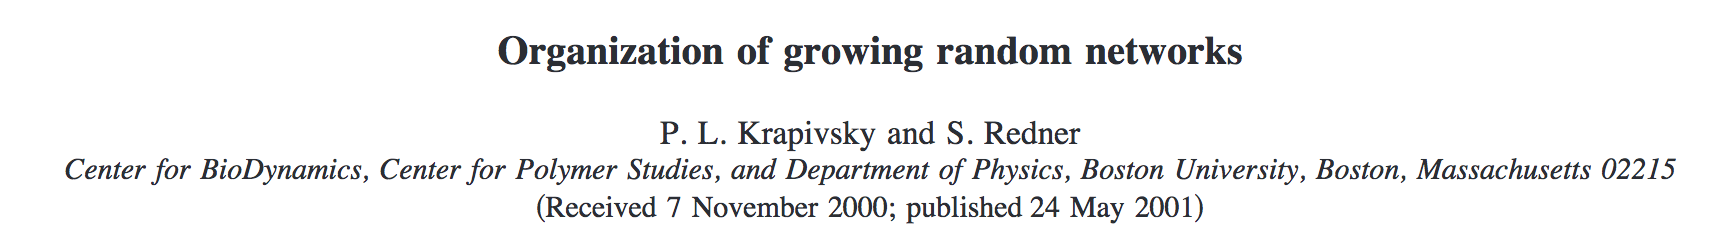
\includegraphics[width=\textwidth]{figures/krapivsky_organization_2001_title}
\end{center}

\begin{itemize}
\item Generalizes preferential attachment process
\end{itemize}

\vfill
\url{https://doi.org/10.1103/PhysRevE.63.066123}

\note{
Only get power law in special case
}

\end{frame}
%%%%%%%%%%%%%%%%%%%%%%%%%%%
\begin{frame}
\frametitle{Modeling}

\begin{center}
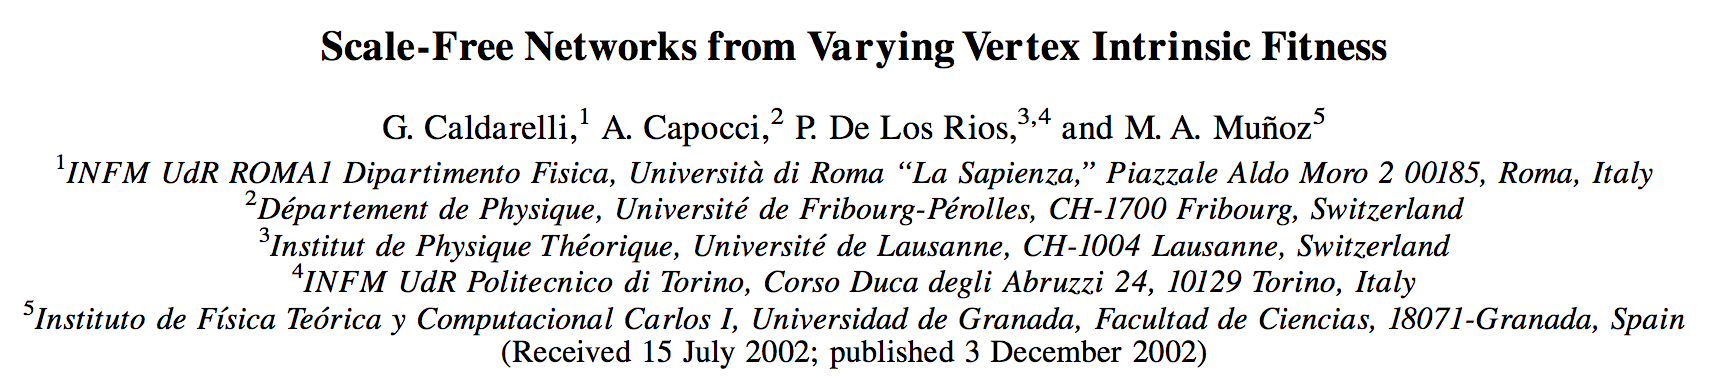
\includegraphics[width=\textwidth]{figures/caldarelli_scale-free_2002_title}
\end{center}

\begin{itemize}
\item power laws can from from ``good-get-richer'' in addition to ``rich-get-richer''
\end{itemize}

\vfill
\url{https://doi.org/10.1103/PhysRevLett.89.258702}

\note{
not rich getting rich
higher quality getting richer
For any given outcome there are often multiple models
}

\end{frame}
%%%%%%%%%%%%%%%%%%%%%%%%%%%
\begin{frame}

Question from previous year:\\
``Is it possible for hubs to exist even where a network doesn't follow a power law distribution? Meaning, the fact that some nodes will be more connected than other nodes, but without the entire network being scale-free?''\\
\pause
A note on terminology:
\begin{itemize}
\item power law
\item scale-free
\item hubs
\end{itemize}

\note{
Clarification of hubs, scale-free, and power law.  In some sense these is ambiguity in the literature here.  In fact my belief is that this is why ``scale-free'' became such a fad.  For a fad ambiguity is good.  Examples: big data and organic foods.  Notice the fight with Jones and Handcock and Liljeros et al.

Let's start with what is defined: power law distributions mean that $p(x) \propto x^{-\alpha}$.

However, make a simple log-log graph is not sufficient to show that something follows a power law. 

And just finding the best fitting $\alpha$ is not sufficient to say that something follows a power law (show McCormick et al paper).  

Scale free is poorly defined.  There is no common scale.  What does that mean?  The largest is 10 times the mean, 100 times the mean, 1,000,000 times the mean?  Scale-free distributions are also sometimes called heavy tailed and sometimes called 80/20 distributions.  For something to be scale-free let's say that there need to some elements that are 1,000 times larger than a typical element.

Hubs is poorly defined, but these would be the things that are particularly large.  In the network of airports, O'Hare is a hub.

Putting all of this together, I would says that the most important point of all of this is variation in connectivity can be important and that variation in connectivity was not something considered by Erdos Reyni or Watts Strogatz.  Also, Barabasi and Albert propose a nice model for where variation in connectivity might come from.
}

\end{frame}
%%%%%%%%%%%%%%%%%%%%%%%%%%%
\begin{frame}

\begin{itemize}
\item growth + preferential attachment $\rightarrow$ power law degree distribution
\pause
\item some (but not all) real networks have a power law degree distribution 
\pause
\item diseases spread more easily on networks with power law degree distribution than on other types of networks
\pause
\item networks with power law degree distribution are robust to random failure but fragile to targeted attack
\end{itemize}


\end{frame}
%%%%%%%%%%%%%%%%%%%%%%%%%%%
\begin{frame}

\begin{itemize}
\item Gladwell, M. (1999). Six degrees of Lois Weisberg. \textit{The New Yorker}.
\item Watts, Chapter 4, 114-129.
\item Feld, S.L. (1981) The focused organization of social ties. \textit{American Journal of Sociology}.
\end{itemize}

\vfill

\includegraphics[width = 0.20\textwidth]{figures/fb_icon.png} {\LARGE $\rightarrow$} 
\includegraphics[width = 0.20\textwidth]{figures/google_plus.png}


\note{Lois Weisberg offers a new way to think about hubs and Feld shows us how non-network things drive tie creation and what that means.

Also, in the next class, I'll explain how these readings predict that you will move from Facebook to Google+}

\end{frame}
%%%%%%%%%%%%%%%%%%%%%%%%%%
\begin{frame}

Please fill out the lecture feedback survey

\end{frame}
%%%%%%%%%%%%%%%%%%%%%%%%%%

\end{document}
